\section{Some Background, some History}\label{sec:ErrorHandlingHistory}
Programmers have to deal with error or failure handling since the first computer was built.

However, the way errors are handled has changed repeatedly over time, yet certain aspects have remained constant.

To demonstrate this, we use a function designed to convert the content of a string into a number. For the sake of simplicity, we allow only integer values in the range of \texttt{-999} to \texttt{+999}. The sign is optional; if it is missing, a positive number is assumed. Leading zeros are permitted. We also assume that the data type for the return value allows only the values from \texttt{-999} to \texttt{+999} – meaning that we have exactly one return value for any valid argument and none for an invalid argument.

The program flowchart for that function is shown on the next page.
\clearpage
\begin{center}
    % dot -Tjpg -y textToNumber.gv > textToNumber.jpg
	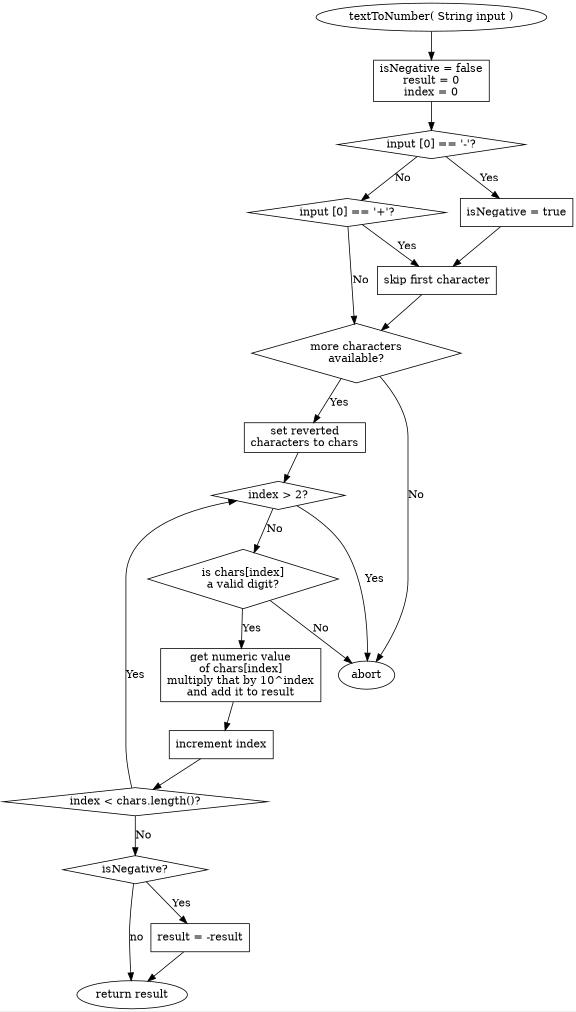
\includegraphics[scale=0.75]{coding/errorHandling/textToNumber}
\end{center}
\clearpage

\keeplisting{16}
The pseudo code for it function would look like this:
\begin{enumerate}[nosep]
	\item{Get the \textit{input} value.}
	\item{If the first character of \textit{input} is \bsq{-}, set the flag \textit{isNegative} to \lstinline|true|, otherwise it is \lstinline|false|.}
    \item{If the first character of \textit{input} is \bsq{+}, skip it.}
    \item{If there are no more characters, abort.}
    \item{Revert the sequence of the remaining characters (\texttt{+123} gets \texttt{321}).}
    \item{Set the \textit{result} to \texttt{0}.}
    \item{Set the \textit{index} to \texttt{0}.}
    \item{If \textit{index} is greater than \texttt{2}, abort.}
    \item{If character on the location determined by \texttt{index} is not a valid digit (something between \texttt{0} and \texttt{9}), abort.}
    \item{Get the numeric value of the character on the location determined by the \textit{index} and multiply that by \texttt{10}\textsuperscript{\textit{index}}.}
    \item{Add that to the \textit{result}.}
    \item{Increment \textit{index}.}
    \item{If \textit{index} is not greater than the number of characters, go back to step~8.}
    \item{If \textit{isNegative} is \lstinline|true|, multiply \textit{result} by \texttt{-1}.}
    \item{Return \textit{result}.}
\end{enumerate}

\keeplisting{23}
We can write this in Java like this:
\begin{lstlisting}
public final int textToNumber( final String input )
{
    var pos = 0;
    var isNegative = false;
    if( input.charAt( pos ) == '-' )
    {
        isNegative = true;
        ++pos;
    }
    else
    {
        if( input.charAt( pos ) == '+' ) ++pos;
    }
    if( pos >= input.length() ) System.exit( -1 );
    final var s = reversed( input.substring( pos ).toCharArray() );
    var result = 0;
    var index = 0;
    while( index < s.length )
    {
        if( index > 2 ) System.exit( -1 );
        if( s [index] < '0' || s [index] > '9' ) System.exit( -1 );
        result += (s [index] - '0') * Math.powExact( 10, index );
        ++index;
    }
    if( isNegative ) result *= -1;
    return result;
}   //  textToNumber()
\end{lstlisting}
Our translation of \bdq{abort} into a call to \lstinline|System.exit()|\index{java.lang!System!exit()} makes the function mostly unusable: it is not really feasible to terminate the current program just because of an invalid input to a data conversion function.

In a language like C\index{C}, we could solve the issue like this:\footnote{Obviously, this is not valid C\index{C} code, but the signature fits the problem.}
\keeplisting{25}
\begin{lstlisting}[language=C]
bool textToNumber( const char* input, int& result )
{
    var pos = 0;
    var isNegative = false;
    if( charAt( input, pos ) == '-' )
    {
        isNegative = true;
        ++pos;
    }
    else
    {
        if( charAt( input, pos ) == '+' ) ++pos;
    }
    if( pos >= length( input ) ) return false; // failed
    var s = reversed( toCharArray( substring( input, pos ) );

    result = 0;
    var index = 0;
    while( index < length( s ) )
    {
        if( index > 2 ) return false; // failed
        if( s [index] < '0' || s [index] > '9' ) return false; // failed
        result += (s [index] - '0') * pow ( 10, index );
        ++index;
    }
    if( isNegative ) result *= -1;

    return true;
}   //  textToNumber()
\end{lstlisting}

You call this method like this:
\begin{lstlisting}[language=C]
int result;
if( !textToNumber( input, &result ) )
{
    // Handle the failure;
}
\end{lstlisting}

The fact that the function's return value must be specified as an argument is not particularly intuitive, but there is no other way to handle it, because none of the possible result values can be co-opted to signal an error.\footnote{You can achieve this also in Java, but it would be even more unintuitive than the C\index{C} version.}

\keeplisting{27}
The Go\index{go} programming language solves this problem by allowing a function to have two return values\footnote{Same as above, this is not valid go\index{go} code, by the signature demonstrates how it would work.}:
\begin{lstlisting}[language=go]
func textToNumber(input string) (bool, int)
{
    var pos = 0;
    var isNegative = false;
    if charAt( input, pos ) == '-' {
        isNegative = true;
        ++pos;
    }
    else
    {
        if charAt( input, pos ) == '+' {++pos}
    }
    if pos >= length( input ) { return false, 0 } // failed
    var s = reversed( toCharArray( substring( input, pos ) );

    result = 0;
    var index = 0;
    while( index < length( s ) )
    {
        if index > 2 { return false, 0 } // failed
        if s [index] < '0' || s [index] > '9' { return false, 0 } // failed
        result += (s [index] - '0') * pow 10, index );
        ++index;
    }
    if isNegative { result *= -1}

    return true, result;
}   //  textToNumber()
\end{lstlisting}

\keeplisting{4}
This is called like this:
\begin{lstlisting}[language=go]
ok, result := textToNumber( input );
if !ok {
    // Handle the failure;
}
\end{lstlisting}

In both cases, we now have a status that tells us whether the function was successful or not – so the reporting aspect is resolved.

If we can be certain that the function call will succeed, we do not need to check the status. However, that would require us to validate the function arguments accordingly, which would merely shift the problem: namely, how do we respond to a failure?

The seemingly simple answer is we jump to an error handler, which then terminates the program. Or, if we are inside a function, we simply return an error status ...

C\index{C} allows us to use \lstinline|goto|, and in go\index{go}, even the standard libraries use \lstinline|goto| to jump to a centralized housekeeping section. However, we must check the returned status for every single method call, which does not necessarily make the code more readable. If the actual return value also needs to be checked – and the execution flow might change as a result – the code quickly becomes completely convoluted.

Not to mention that for both C\index{C} and go\index{go}, the \lstinline|goto| allows us to jump only to a label inside the current function, but not to a global error handler.

\keeplisting{28}
To avoid this problem, Java uses Exceptions\index{exception} to report failures.\footnote{Java is not the only language that uses Exceptions\index{exception}, and it was not the first. But is seen as the first that introduced \lstinline|finally|.} A more sensible Java version of our function would therefore look like this:
\begin{lstlisting}
public final int textToNumber( final String input )
{
    var pos = 0;
    var isNegative = false;
    if( input.charAt( pos ) == '-' )
    {
        isNegative = true;
        ++pos;
    }
    else
    {
        if( input.charAt( pos ) == '+' ) ++pos;
    }
    if( pos >= input.length() ) throw new RuntimeException( "No more characters" );
    final var s = reversed( input.substring( pos ).toCharArray() );

    var result = 0;
    var index = 0;
    while( index < s.length )
    {
        if( index > 2 ) throw new RuntimeException( "Too many digits" );
        if( s [index] < '0' || s [index] > '9' )  throw new RuntimeException( "Invalid character: " + s [index] );
        result += (s [index] - '0') * Math.powExact( 10, index );
        ++index;
    }
    if( isNegative ) result *= -1;

    return result;
}   //  textToNumber()
\end{lstlisting}

\keeplisting{8}
If you want to deal with the failure, you will call \lstinline|textToNumber()| like this:
\begin{lstlisting}
try
{
    final var number = textToNumber( text );
}
catch( final RuntimeException e )
{
    // Handle the exception
}
\end{lstlisting}

If we want to delegate that failure to a higher level, we just call \lstinline|textToNumber()|, and ignore the exception\index{exception}; it \textit{bubbles up} automatically:
\begin{lstlisting}
final var number = textToNumber( text );
\end{lstlisting}

Looks like the perfect solution to our problem. Unfortunately, there is nothing like a free lunch, as we will see in the \hyperref[sec:ExceptionCosts]{next} chapter.

%==============================================================================
% End of file!!
%==============================================================================
